\documentclass[11pt, letterpaper]{article}

% Fonts and Encoding
\usepackage[utf8]{inputenc}
\usepackage[T1]{fontenc}
\usepackage{lmodern} % High-quality Latin Modern vector font

% Math and Symbols
\usepackage{amsmath, amssymb, amsthm, amsfonts, mathrsfs, mathtools}

% Layout and Geometry
\usepackage{geometry}
\geometry{letterpaper, margin=1in}
\setlength{\parindent}{0pt}
\setlength{\parskip}{0.6em}

% Formatting and Graphics
\usepackage{graphicx, xcolor, enumitem, booktabs, array, tabularx}

% TikZ for Illustrations
\usepackage{tikz}
\usetikzlibrary{arrows.meta, positioning, shapes.geometric, calc, backgrounds, matrix}

% Clickable Links and TOC
\usepackage{hyperref}
\hypersetup{
    colorlinks=true,
    linkcolor=blue,
    filecolor=magenta,      
    urlcolor=cyan,
    pdftitle={Transforms of Discontinuous Functions},
}

% Theorem Environments
\newtheorem{theorem}{Theorem}[section]
\newtheorem{lemma}[theorem]{Lemma}
\newtheorem{proposition}[theorem]{Proposition}
\newtheorem{corollary}[theorem]{Corollary}
\theoremstyle{definition}
\newtheorem{definition}{Definition}[section]
\newtheorem{axiom}{Axiom}[section]
\newtheorem{example}{Example}[section]
\theoremstyle{remark}
\newtheorem{remark}{Remark}[section]

% Custom Commands (Enforced standard notation)
\newcommand{\R}{\mathbb{R}}
\newcommand{\N}{\mathbb{N}}
\newcommand{\Z}{\mathbb{Z}}
\newcommand{\Q}{\mathbb{Q}}
\newcommand{\E}{\mathbb{E}}
\newcommand{\Prob}{\mathbb{P}}
\newcommand{\F}{\mathcal{F}}
\newcommand{\Lap}{\mathcal{L}}

\title{\textbf{Transforms of Discontinuous Functions\\Problem Sets and Detailed Solutions}}
\author{Tashfeen Omran}
\date{\today}

\begin{document}

\maketitle
\tableofcontents
\newpage

\section{Concept Checklist \& Question Mapping}

The following table outlines the core concepts and problem types associated with the Laplace transforms of discontinuous functions, mapped directly to the curated problem sets.

\renewcommand{\arraystretch}{1.5}
\begin{tabularx}{\textwidth}{@{} l X >{$\displaystyle}c<{$} @{}}
\toprule
\textbf{ID} & \textbf{Concept / Problem Type} & \text{\textbf{Questions}} \\
\midrule
C1 & Expressing Piecewise Functions using Step Functions & 1 - 4 \\
C2 & Direct Laplace Transforms of Discontinuous Functions & 5 - 10 \\
C3 & Inverse Laplace Transforms using the Second Shifting Theorem & 11 - 16 \\
C4 & Solving First-Order IVPs with Discontinuous Forcing & 17 - 20 \\
C5 & Solving Second-Order IVPs with Discontinuous Forcing & 21 - 26 \\
C6 & Applications: RLC Circuits & 27 - 28 \\
C7 & Applications: Mixing Tanks & 29 - 30 \\
\bottomrule
\end{tabularx}

\vspace{1em}
\textbf{Key Techniques Tested:}
\begin{itemize}
    \item \textbf{The Add and Subtract Trick:} Algebraically manipulating $t$ to match the shift $(t-a)$.
    \item \textbf{Trigonometric Periodicity:} Utilizing periods of sine and cosine to simplify shifts (e.g., $\sin(t - \pi) = -\sin(t)$).
    \item \textbf{Heavy Partial Fraction Decomposition (PFD):} Breaking down complex $s$-domain expressions.
    \item \textbf{The $H(s)$ Isolation Method:} Separating the exponential shift $e^{-as}$ from the rational function $H(s)$ to prevent algebraic errors during inversion.
\end{itemize}

\newpage

\section{Problem Sets}

\subsection{C1: Expressing Piecewise Functions}
\textbf{1.} Sketch the graph and express the following function using Heaviside step functions: $f(t) = 4$ for $0 < t < 3$, and $f(t) = 0$ for $t > 3$. \\
\textbf{2.} Sketch the graph and express the following function using Heaviside step functions: $f(t) = 2t$ for $0 < t < 2$, and $f(t) = 4$ for $t > 2$. \\
\textbf{3.} Express the piecewise function $f(t)$ in terms of step functions: $f(t) = e^{2t}$ for $0 < t < 1$, and $f(t) = e^{-2t}$ for $t > 1$. \\
\textbf{4.} Express the piecewise function $f(t)$ in terms of step functions: $f(t) = \cos(3t)$ for $0 < t < \pi$, and $f(t) = 0$ for $t > \pi$.

\subsection{C2: Direct Laplace Transforms}
\textbf{5.} Determine the Laplace transform of $f(t) = (t-2)^3 u(t-2)$. \\
\textbf{6.} Determine the Laplace transform of $f(t) = t^2 u(t-1)$. \\
\textbf{7.} Determine the Laplace transform of $f(t) = e^{3t} u(t-2)$. \\
\textbf{8.} Determine the Laplace transform of $f(t) = \sin(2t) u(t-\pi/4)$. \\
\textbf{9.} Determine the Laplace transform of $f(t) = (t^2 - 3t + 2) u(t-3)$. \\
\textbf{10.} Determine the Laplace transform of $f(t)$, where $f(t) = 2$ for $0 < t < 2$, and $f(t) = t$ for $t > 2$.

\subsection{C3: Inverse Laplace Transforms}
\textbf{11.} Find the inverse Laplace transform: $\Lap^{-1} \left\{ \frac{e^{-3s}}{s^4} \right\}$. \\
\textbf{12.} Find the inverse Laplace transform: $\Lap^{-1} \left\{ \frac{e^{-s}}{s-4} \right\}$. \\
\textbf{13.} Find the inverse Laplace transform: $\Lap^{-1} \left\{ \frac{s e^{-2\pi s}}{s^2 + 9} \right\}$. \\
\textbf{14.} Find the inverse Laplace transform: $\Lap^{-1} \left\{ \frac{e^{-2s}}{s^2 + 4s + 13} \right\}$. \\
\textbf{15.} Find the inverse Laplace transform: $\Lap^{-1} \left\{ \frac{e^{-s}(s+2)}{s^2 + 3s + 2} \right\}$. \\
\textbf{16.} Find the inverse Laplace transform: $\Lap^{-1} \left\{ \frac{2 - e^{-3s}}{s^2} \right\}$.

\subsection{C4: First-Order Initial Value Problems}
\textbf{17.} Solve the IVP: $y' + 2y = u(t-1)$, with $y(0) = 1$. \\
\textbf{18.} Solve the IVP: $y' - y = 2u(t-2)$, with $y(0) = 0$. \\
\textbf{19.} Solve the IVP: $y' + 4y = t u(t-1)$, with $y(0) = 0$. \\
\textbf{20.} Solve the IVP: $y' + y = \cos(t) u(t-\pi)$, with $y(0) = 1$.

\subsection{C5: Second-Order Initial Value Problems}
\textbf{21.} Solve the IVP: $y'' + 4y = u(t-2)$, with $y(0) = 0, y'(0) = 0$. \\
\textbf{22.} Solve the IVP: $y'' - 9y = u(t-1) - u(t-3)$, with $y(0) = 0, y'(0) = 0$. \\
\textbf{23.} Solve the IVP: $y'' + y = \sin(3t) u(t-\pi)$, with $y(0) = 0, y'(0) = 0$. \\
\textbf{24.} Solve the IVP: $y'' + 4y' + 4y = u(t-2)$, with $y(0) = 1, y'(0) = 0$. \\
\textbf{25.} Solve the IVP: $y'' + 16y = t u(t-1)$, with $y(0) = 0, y'(0) = 0$. \\
\textbf{26.} Solve the IVP: $y'' + 5y' + 6y = u(t-2)$, with $y(0) = 0, y'(0) = 1$.

\subsection{C6: Applications - RLC Circuits}
\textbf{27.} An RLC circuit is governed by $I'' + 6I' + 9I = 18u(t-1)$. Find the current $I(t)$ if $I(0) = 0$ and $I'(0) = 0$. \\
\textbf{28.} An RLC circuit is governed by $I'' + 2I' + 10I = 20u(t-\pi) - 20u(t-2\pi)$. Find the current $I(t)$ if $I(0) = 0$ and $I'(0) = 0$.

\subsection{C7: Applications - Mixing Tanks}
\textbf{29.} A tank initially contains $200$ L of pure water. A salt solution is pumped in at $10$ L/min. The concentration of the incoming solution is $0.5$ kg/L for the first $5$ minutes, and then pure water is pumped in thereafter. The well-mixed solution is pumped out at $10$ L/min. Find the amount of salt $x(t)$ in the tank at any time $t$. \\
\textbf{30.} A tank initially contains $100$ L of water with $5$ kg of dissolved salt. Pure water is pumped in at $2$ L/min for the first $10$ minutes. After $10$ minutes, a salt solution with a concentration of $4$ kg/L is pumped in at the same rate. The well-mixed solution is pumped out at $2$ L/min. Find the amount of salt $x(t)$ in the tank at any time $t$.

\newpage

\section{Detailed Solutions}

\subsection{C1: Expressing Piecewise Functions}

\textbf{Problem 1:} Sketch the graph and express the following function using Heaviside step functions: $f(t) = 4$ for $0 < t < 3$, and $f(t) = 0$ for $t > 3$.

\textbf{Solution:}
The function "turns on" at $t=0$ with a value of $4$ and "turns off" at $t=3$. We can express this using a rectangular window function.
\[ f(t) = 4(u(t) - u(t-3)) = 4 - 4u(t-3) \]

\begin{center}
\begin{tikzpicture}[scale=1.5]
    % Background fill to ensure layering
    \fill[white] (-0.5, -0.5) rectangle (5.5, 5.5);
    
    % Grid and Axes
    \draw[thin, gray!30] (-0.5, -0.5) grid (4.5, 5.5);
    \draw[->, thick] (-0.5, 0) -- (4.5, 0) node[right] {$t$};
    \draw[->, thick] (0, -0.5) -- (0, 5.5) node[above] {$f(t)$};
    
    % Ticks
    \draw[thick] (3, 0) -- (3, -0.1) node[below=2pt] {$3$};
    \draw[thick] (0, 4) -- (-0.1, 4) node[left=2pt] {$4$};
    
    % Plot
    \draw[ultra thick, blue!80!black] (0, 4) -- (3, 4);
    \draw[ultra thick, blue!80!black] (3, 0) -- (4.2, 0);
    \draw[blue!80!black, fill=white, thick] (3, 4) circle (1.5pt);
    \draw[blue!80!black, fill=blue!80!black] (3, 0) circle (1.5pt);
    
    % Annotation
    \node[align=left, anchor=west, inner sep=8pt, text=black] at (4.5, 4) {
        $\displaystyle f(t) = 4[u(t) - u(t-3)]$\\[4pt]
        Rectangular Window
    };
\end{tikzpicture}
\end{center}

\vspace{1em}
\textbf{Problem 2:} Sketch the graph and express the following function using Heaviside step functions: $f(t) = 2t$ for $0 < t < 2$, and $f(t) = 4$ for $t > 2$.

\textbf{Solution:}
The function starts as $2t$. At $t=2$, we must "turn off" $2t$ and "turn on" $4$.
\[ f(t) = 2t + (4 - 2t)u(t-2) \]

\begin{center}
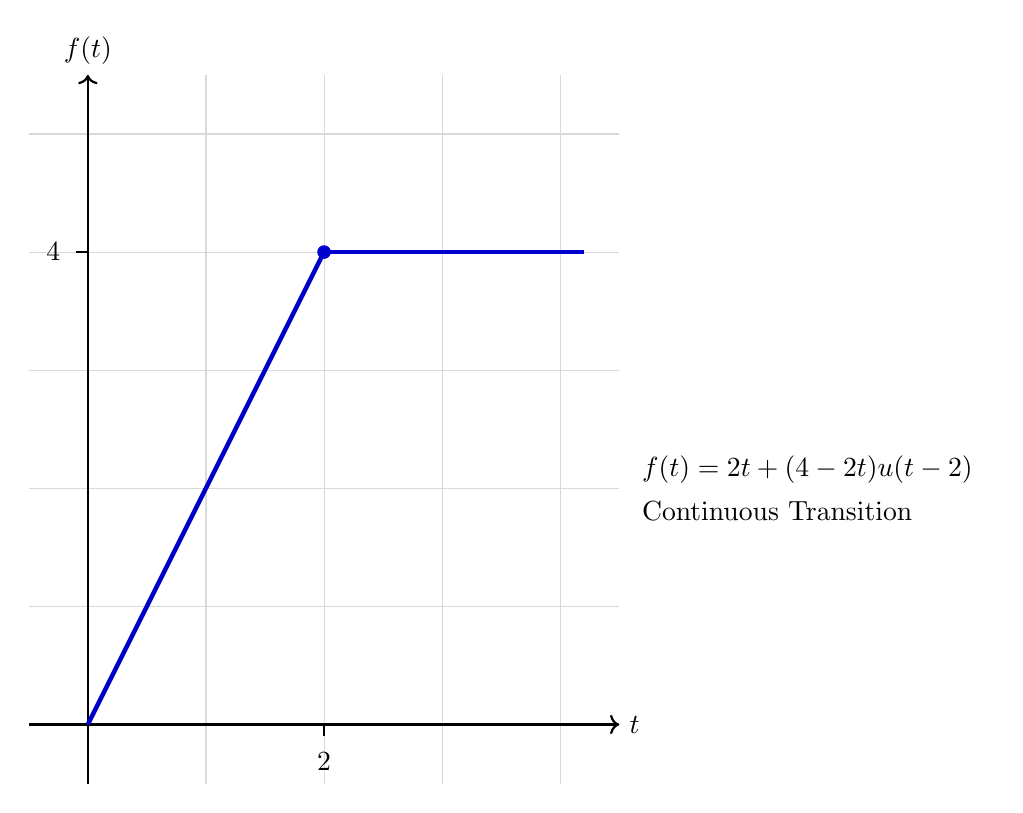
\begin{tikzpicture}[scale=1.5]
    % Background fill
    \fill[white] (-0.5, -0.5) rectangle (5.5, 5.5);
    
    % Grid and Axes
    \draw[thin, gray!30] (-0.5, -0.5) grid (4.5, 5.5);
    \draw[->, thick] (-0.5, 0) -- (4.5, 0) node[right] {$t$};
    \draw[->, thick] (0, -0.5) -- (0, 5.5) node[above] {$f(t)$};
    
    % Ticks
    \draw[thick] (2, 0) -- (2, -0.1) node[below=2pt] {$2$};
    \draw[thick] (0, 4) -- (-0.1, 4) node[left=2pt] {$4$};
    
    % Plot
    \draw[ultra thick, blue!80!black] (0, 0) -- (2, 4);
    \draw[ultra thick, blue!80!black] (2, 4) -- (4.2, 4);
    \draw[blue!80!black, fill=blue!80!black] (2, 4) circle (1.5pt);
    
    % Annotation
    \node[align=left, anchor=west, inner sep=8pt, text=black] at (4.5, 2) {
        $\displaystyle f(t) = 2t + (4 - 2t)u(t-2)$\\[4pt]
        Continuous Transition
    };
\end{tikzpicture}
\end{center}

\vspace{1em}
\textbf{Problem 3:} Express the piecewise function $f(t)$ in terms of step functions: $f(t) = e^{2t}$ for $0 < t < 1$, and $f(t) = e^{-2t}$ for $t > 1$.

\textbf{Solution:}
We start with $e^{2t}$. At $t=1$, we subtract $e^{2t}$ and add $e^{-2t}$.
\[ f(t) = e^{2t} + (e^{-2t} - e^{2t})u(t-1) \]

\vspace{1em}
\textbf{Problem 4:} Express the piecewise function $f(t)$ in terms of step functions: $f(t) = \cos(3t)$ for $0 < t < \pi$, and $f(t) = 0$ for $t > \pi$.

\textbf{Solution:}
We start with $\cos(3t)$. At $t=\pi$, we subtract it to bring the function to $0$.
\[ f(t) = \cos(3t) - \cos(3t)u(t-\pi) \]

\subsection{C2: Direct Laplace Transforms}

\textbf{Problem 5:} Determine the Laplace transform of $f(t) = (t-2)^3 u(t-2)$.

\textbf{Solution:}
Using the Second Shifting Theorem $\Lap\{g(t-a)u(t-a)\} = e^{-as}G(s)$, where $g(t) = t^3$ and $a = 2$:
\[ \Lap\{(t-2)^3 u(t-2)\} = e^{-2s} \Lap\{t^3\} = e^{-2s} \left( \frac{3!}{s^4} \right) = \frac{6e^{-2s}}{s^4} \]

\vspace{1em}
\textbf{Problem 6:} Determine the Laplace transform of $f(t) = t^2 u(t-1)$.

\textbf{Solution:}
Using the practical computation formula $\Lap\{g(t)u(t-a)\} = e^{-as}\Lap\{g(t+a)\}$, with $g(t) = t^2$ and $a = 1$:
\[ g(t+1) = (t+1)^2 = t^2 + 2t + 1 \]
\[ \Lap\{t^2 u(t-1)\} = e^{-s} \Lap\{t^2 + 2t + 1\} = e^{-s} \left( \frac{2}{s^3} + \frac{2}{s^2} + \frac{1}{s} \right) \]

\vspace{1em}
\textbf{Problem 7:} Determine the Laplace transform of $f(t) = e^{3t} u(t-2)$.

\textbf{Solution:}
Using $\Lap\{g(t)u(t-a)\} = e^{-as}\Lap\{g(t+a)\}$ with $g(t) = e^{3t}$ and $a = 2$:
\[ g(t+2) = e^{3(t+2)} = e^{3t}e^6 \]
\[ \Lap\{e^{3t} u(t-2)\} = e^{-2s} \Lap\{e^6 e^{3t}\} = e^{-2s} e^6 \Lap\{e^{3t}\} = \frac{e^{6-2s}}{s-3} \]

\vspace{1em}
\textbf{Problem 8:} Determine the Laplace transform of $f(t) = \sin(2t) u(t-\pi/4)$.

\textbf{Solution:}
Using $\Lap\{g(t)u(t-a)\} = e^{-as}\Lap\{g(t+a)\}$ with $g(t) = \sin(2t)$ and $a = \pi/4$:
\[ g(t+\pi/4) = \sin\left(2\left(t + \frac{\pi}{4}\right)\right) = \sin\left(2t + \frac{\pi}{2}\right) = \cos(2t) \]
\[ \Lap\{\sin(2t) u(t-\pi/4)\} = e^{-\pi s / 4} \Lap\{\cos(2t)\} = \frac{s e^{-\pi s / 4}}{s^2 + 4} \]

\vspace{1em}
\textbf{Problem 9:} Determine the Laplace transform of $f(t) = (t^2 - 3t + 2) u(t-3)$.

\textbf{Solution:}
Using $\Lap\{g(t)u(t-a)\} = e^{-as}\Lap\{g(t+a)\}$ with $g(t) = t^2 - 3t + 2$ and $a = 3$:
\begin{align*}
g(t+3) &= (t+3)^2 - 3(t+3) + 2 \\
&= (t^2 + 6t + 9) - 3t - 9 + 2 \\
&= t^2 + 3t + 2
\end{align*}
\[ \Lap\{(t^2 - 3t + 2) u(t-3)\} = e^{-3s} \Lap\{t^2 + 3t + 2\} = e^{-3s} \left( \frac{2}{s^3} + \frac{3}{s^2} + \frac{2}{s} \right) \]

\vspace{1em}
\textbf{Problem 10:} Determine the Laplace transform of $f(t)$, where $f(t) = 2$ for $0 < t < 2$, and $f(t) = t$ for $t > 2$.

\textbf{Solution:}
First, express $f(t)$ using step functions:
\[ f(t) = 2 + (t - 2)u(t-2) \]
Now, take the Laplace transform directly:
\[ \Lap\{f(t)\} = \Lap\{2\} + \Lap\{(t-2)u(t-2)\} = \frac{2}{s} + \frac{e^{-2s}}{s^2} \]

\subsection{C3: Inverse Laplace Transforms}

\textbf{Problem 11:} Find the inverse Laplace transform: $\Lap^{-1} \left\{ \frac{e^{-3s}}{s^4} \right\}$.

\textbf{Solution:}
Let $F(s) = \frac{1}{s^4}$. The inverse transform is $f(t) = \frac{t^3}{3!} = \frac{t^3}{6}$.
Using the inverse translation theorem $\Lap^{-1}\{e^{-as}F(s)\} = f(t-a)u(t-a)$:
\[ \Lap^{-1} \left\{ \frac{e^{-3s}}{s^4} \right\} = \frac{1}{6}(t-3)^3 u(t-3) \]

\vspace{1em}
\textbf{Problem 12:} Find the inverse Laplace transform: $\Lap^{-1} \left\{ \frac{e^{-s}}{s-4} \right\}$.

\textbf{Solution:}
Let $F(s) = \frac{1}{s-4} \implies f(t) = e^{4t}$.
Applying the shift $t \to t-1$:
\[ \Lap^{-1} \left\{ \frac{e^{-s}}{s-4} \right\} = e^{4(t-1)} u(t-1) \]

\vspace{1em}
\textbf{Problem 13:} Find the inverse Laplace transform: $\Lap^{-1} \left\{ \frac{s e^{-2\pi s}}{s^2 + 9} \right\}$.

\textbf{Solution:}
Let $F(s) = \frac{s}{s^2+9} \implies f(t) = \cos(3t)$.
Applying the shift $t \to t-2\pi$:
\[ \Lap^{-1} \left\{ \frac{s e^{-2\pi s}}{s^2 + 9} \right\} = \cos(3(t-2\pi)) u(t-2\pi) \]
By trigonometric periodicity, $\cos(3t - 6\pi) = \cos(3t)$, so:
\[ \Lap^{-1} \left\{ \frac{s e^{-2\pi s}}{s^2 + 9} \right\} = \cos(3t) u(t-2\pi) \]

\vspace{1em}
\textbf{Problem 14:} Find the inverse Laplace transform: $\Lap^{-1} \left\{ \frac{e^{-2s}}{s^2 + 4s + 13} \right\}$.

\textbf{Solution:}
First, complete the square for the denominator: $s^2 + 4s + 13 = (s+2)^2 + 9$.
Let $F(s) = \frac{1}{(s+2)^2 + 9} = \frac{1}{3} \frac{3}{(s+2)^2 + 3^2} \implies f(t) = \frac{1}{3} e^{-2t} \sin(3t)$.
Applying the shift $t \to t-2$:
\[ \Lap^{-1} \left\{ \frac{e^{-2s}}{s^2 + 4s + 13} \right\} = \frac{1}{3} e^{-2(t-2)} \sin(3(t-2)) u(t-2) \]

\vspace{1em}
\textbf{Problem 15:} Find the inverse Laplace transform: $\Lap^{-1} \left\{ \frac{e^{-s}(s+2)}{s^2 + 3s + 2} \right\}$.

\textbf{Solution:}
Factor the denominator: $s^2 + 3s + 2 = (s+1)(s+2)$.
Let $F(s) = \frac{s+2}{(s+1)(s+2)} = \frac{1}{s+1} \implies f(t) = e^{-t}$.
Applying the shift $t \to t-1$:
\[ \Lap^{-1} \left\{ \frac{e^{-s}(s+2)}{s^2 + 3s + 2} \right\} = e^{-(t-1)} u(t-1) \]

\vspace{1em}
\textbf{Problem 16:} Find the inverse Laplace transform: $\Lap^{-1} \left\{ \frac{2 - e^{-3s}}{s^2} \right\}$.

\textbf{Solution:}
Split the expression:
\[ \Lap^{-1} \left\{ \frac{2}{s^2} - \frac{e^{-3s}}{s^2} \right\} = 2t - (t-3)u(t-3) \]

\subsection{C4: First-Order Initial Value Problems}

\textbf{Problem 17:} Solve the IVP: $y' + 2y = u(t-1)$, with $y(0) = 1$.

\textbf{Solution:}
Take the Laplace transform of both sides:
\[ (sY(s) - 1) + 2Y(s) = \frac{e^{-s}}{s} \]
\[ (s+2)Y(s) = 1 + \frac{e^{-s}}{s} \]
\[ Y(s) = \frac{1}{s+2} + \frac{e^{-s}}{s(s+2)} \]
Let $H(s) = \frac{1}{s(s+2)}$. Using PFD:
\[ \frac{1}{s(s+2)} = \frac{1/2}{s} - \frac{1/2}{s+2} \implies h(t) = \frac{1}{2} - \frac{1}{2}e^{-2t} \]
Inverting $Y(s)$:
\[ y(t) = e^{-2t} + h(t-1)u(t-1) = e^{-2t} + \left( \frac{1}{2} - \frac{1}{2}e^{-2(t-1)} \right) u(t-1) \]

\vspace{1em}
\textbf{Problem 18:} Solve the IVP: $y' - y = 2u(t-2)$, with $y(0) = 0$.

\textbf{Solution:}
Take the Laplace transform:
\[ sY(s) - Y(s) = \frac{2e^{-2s}}{s} \]
\[ Y(s) = \frac{2e^{-2s}}{s(s-1)} \]
Let $H(s) = \frac{2}{s(s-1)} = \frac{2}{s-1} - \frac{2}{s} \implies h(t) = 2e^t - 2$.
Inverting $Y(s)$:
\[ y(t) = h(t-2)u(t-2) = (2e^{t-2} - 2)u(t-2) \]

\vspace{1em}
\textbf{Problem 19:} Solve the IVP: $y' + 4y = t u(t-1)$, with $y(0) = 0$.

\textbf{Solution:}
First, transform the right side using the "Add and Subtract" trick:
\[ \Lap\{t u(t-1)\} = e^{-s}\Lap\{t+1\} = e^{-s} \left( \frac{1}{s^2} + \frac{1}{s} \right) = e^{-s} \frac{s+1}{s^2} \]
Transform the DE:
\[ (s+4)Y(s) = e^{-s} \frac{s+1}{s^2} \implies Y(s) = e^{-s} \frac{s+1}{s^2(s+4)} \]
Let $H(s) = \frac{s+1}{s^2(s+4)}$. Using PFD:
\[ \frac{s+1}{s^2(s+4)} = \frac{A}{s} + \frac{B}{s^2} + \frac{C}{s+4} \]
\[ A s(s+4) + B(s+4) + C s^2 = s+1 \]
Setting $s=0 \implies 4B = 1 \implies B = 1/4$. \\
Setting $s=-4 \implies 16C = -3 \implies C = -3/16$. \\
Comparing $s^2$ coefficients: $A + C = 0 \implies A = 3/16$.
\[ H(s) = \frac{3/16}{s} + \frac{1/4}{s^2} - \frac{3/16}{s+4} \implies h(t) = \frac{3}{16} + \frac{1}{4}t - \frac{3}{16}e^{-4t} \]
Inverting $Y(s)$:
\[ y(t) = h(t-1)u(t-1) = \left( \frac{3}{16} + \frac{1}{4}(t-1) - \frac{3}{16}e^{-4(t-1)} \right) u(t-1) \]

\vspace{1em}
\textbf{Problem 20:} Solve the IVP: $y' + y = \cos(t) u(t-\pi)$, with $y(0) = 1$.

\textbf{Solution:}
Using trigonometric periodicity, $\cos(t) = -\cos(t-\pi)$.
\[ \Lap\{\cos(t) u(t-\pi)\} = \Lap\{-\cos(t-\pi) u(t-\pi)\} = -e^{-\pi s} \frac{s}{s^2+1} \]
Transform the DE:
\[ (s+1)Y(s) - 1 = -e^{-\pi s} \frac{s}{s^2+1} \]
\[ Y(s) = \frac{1}{s+1} - e^{-\pi s} \frac{s}{(s+1)(s^2+1)} \]
Let $H(s) = \frac{s}{(s+1)(s^2+1)}$. Using PFD:
\[ \frac{s}{(s+1)(s^2+1)} = \frac{A}{s+1} + \frac{Bs+C}{s^2+1} \]
\[ A(s^2+1) + (Bs+C)(s+1) = s \]
Setting $s=-1 \implies 2A = -1 \implies A = -1/2$. \\
Comparing $s^2$ coefficients: $A + B = 0 \implies B = 1/2$. \\
Comparing constants: $A + C = 0 \implies C = 1/2$.
\[ H(s) = -\frac{1/2}{s+1} + \frac{1}{2} \frac{s}{s^2+1} + \frac{1}{2} \frac{1}{s^2+1} \implies h(t) = -\frac{1}{2}e^{-t} + \frac{1}{2}\cos(t) + \frac{1}{2}\sin(t) \]
Inverting $Y(s)$:
\[ y(t) = e^{-t} - h(t-\pi)u(t-\pi) \]
Since $\cos(t-\pi) = -\cos(t)$ and $\sin(t-\pi) = -\sin(t)$:
\[ h(t-\pi) = -\frac{1}{2}e^{-(t-\pi)} - \frac{1}{2}\cos(t) - \frac{1}{2}\sin(t) \]
\[ y(t) = e^{-t} + \left( \frac{1}{2}e^{-(t-\pi)} + \frac{1}{2}\cos(t) + \frac{1}{2}\sin(t) \right) u(t-\pi) \]

\subsection{C5: Second-Order Initial Value Problems}

\textbf{Problem 21:} Solve the IVP: $y'' + 4y = u(t-2)$, with $y(0) = 0, y'(0) = 0$.

\textbf{Solution:}
Transform the DE:
\[ (s^2+4)Y(s) = \frac{e^{-2s}}{s} \implies Y(s) = \frac{e^{-2s}}{s(s^2+4)} \]
Let $H(s) = \frac{1}{s(s^2+4)} = \frac{1/4}{s} - \frac{1/4 \cdot s}{s^2+4} \implies h(t) = \frac{1}{4} - \frac{1}{4}\cos(2t)$.
Inverting $Y(s)$:
\[ y(t) = h(t-2)u(t-2) = \left( \frac{1}{4} - \frac{1}{4}\cos(2(t-2)) \right) u(t-2) \]

\vspace{1em}
\textbf{Problem 22:} Solve the IVP: $y'' - 9y = u(t-1) - u(t-3)$, with $y(0) = 0, y'(0) = 0$.

\textbf{Solution:}
Transform the DE:
\[ (s^2-9)Y(s) = \frac{e^{-s}}{s} - \frac{e^{-3s}}{s} \implies Y(s) = \frac{e^{-s} - e^{-3s}}{s(s^2-9)} \]
Let $H(s) = \frac{1}{s(s^2-9)} = \frac{1}{s(s-3)(s+3)}$. Using PFD:
\[ \frac{1}{s(s-3)(s+3)} = \frac{-1/9}{s} + \frac{1/18}{s-3} + \frac{1/18}{s+3} \]
\[ h(t) = -\frac{1}{9} + \frac{1}{18}e^{3t} + \frac{1}{18}e^{-3t} = \frac{1}{9}(\cosh(3t) - 1) \]
Inverting $Y(s)$:
\[ y(t) = h(t-1)u(t-1) - h(t-3)u(t-3) \]

\vspace{1em}
\textbf{Problem 23:} Solve the IVP: $y'' + y = \sin(3t) u(t-\pi)$, with $y(0) = 0, y'(0) = 0$.

\textbf{Solution:}
Using trigonometric periodicity, $\sin(3t) = \sin(3(t-\pi+\pi)) = \sin(3(t-\pi) + 3\pi) = -\sin(3(t-\pi))$.
\[ \Lap\{\sin(3t) u(t-\pi)\} = -e^{-\pi s} \frac{3}{s^2+9} \]
Transform the DE:
\[ (s^2+1)Y(s) = -e^{-\pi s} \frac{3}{s^2+9} \implies Y(s) = -e^{-\pi s} \frac{3}{(s^2+1)(s^2+9)} \]
Let $H(s) = \frac{3}{(s^2+1)(s^2+9)}$. Using PFD:
\[ \frac{3}{(s^2+1)(s^2+9)} = \frac{A}{s^2+1} + \frac{B}{s^2+9} \]
\[ A(s^2+9) + B(s^2+1) = 3 \implies A+B=0, \ 9A+B=3 \implies 8A=3 \implies A=3/8, B=-3/8 \]
\[ H(s) = \frac{3/8}{s^2+1} - \frac{3/8}{s^2+9} = \frac{3}{8}\frac{1}{s^2+1} - \frac{1}{8}\frac{3}{s^2+9} \implies h(t) = \frac{3}{8}\sin(t) - \frac{1}{8}\sin(3t) \]
Inverting $Y(s)$:
\[ y(t) = -h(t-\pi)u(t-\pi) = -\left( \frac{3}{8}\sin(t-\pi) - \frac{1}{8}\sin(3(t-\pi)) \right) u(t-\pi) \]
Since $\sin(t-\pi) = -\sin(t)$ and $\sin(3(t-\pi)) = -\sin(3t)$:
\[ y(t) = \left( \frac{3}{8}\sin(t) - \frac{1}{8}\sin(3t) \right) u(t-\pi) \]

\vspace{1em}
\textbf{Problem 24:} Solve the IVP: $y'' + 4y' + 4y = u(t-2)$, with $y(0) = 1, y'(0) = 0$.

\textbf{Solution:}
Transform the DE:
\[ (s^2+4s+4)Y(s) - s - 4 = \frac{e^{-2s}}{s} \]
\[ Y(s) = \frac{s+4}{(s+2)^2} + \frac{e^{-2s}}{s(s+2)^2} \]
First term: $\frac{s+2+2}{(s+2)^2} = \frac{1}{s+2} + \frac{2}{(s+2)^2} \implies e^{-2t} + 2te^{-2t}$. \\
Let $H(s) = \frac{1}{s(s+2)^2}$. Using PFD:
\[ \frac{1}{s(s+2)^2} = \frac{A}{s} + \frac{B}{s+2} + \frac{C}{(s+2)^2} \]
\[ A(s+2)^2 + Bs(s+2) + Cs = 1 \]
Setting $s=0 \implies 4A = 1 \implies A = 1/4$. \\
Setting $s=-2 \implies -2C = 1 \implies C = -1/2$. \\
Comparing $s^2$ coefficients: $A + B = 0 \implies B = -1/4$.
\[ h(t) = \frac{1}{4} - \frac{1}{4}e^{-2t} - \frac{1}{2}te^{-2t} \]
Inverting $Y(s)$:
\[ y(t) = e^{-2t} + 2te^{-2t} + h(t-2)u(t-2) \]

\vspace{1em}
\textbf{Problem 25:} Solve the IVP: $y'' + 16y = t u(t-1)$, with $y(0) = 0, y'(0) = 0$.

\textbf{Solution:}
Transform the right side: $\Lap\{t u(t-1)\} = e^{-s}\Lap\{t+1\} = e^{-s} \frac{s+1}{s^2}$.
Transform the DE:
\[ (s^2+16)Y(s) = e^{-s} \frac{s+1}{s^2} \implies Y(s) = e^{-s} \frac{s+1}{s^2(s^2+16)} \]
Let $H(s) = \frac{s+1}{s^2(s^2+16)}$. Using PFD:
\[ \frac{s+1}{s^2(s^2+16)} = \frac{As+B}{s^2} + \frac{Cs+D}{s^2+16} \]
\[ (As+B)(s^2+16) + (Cs+D)s^2 = s+1 \]
\[ As^3 + 16As + Bs^2 + 16B + Cs^3 + Ds^2 = s+1 \]
Comparing coefficients:
$16B = 1 \implies B = 1/16$. \\
$16A = 1 \implies A = 1/16$. \\
$A+C = 0 \implies C = -1/16$. \\
$B+D = 0 \implies D = -1/16$.
\[ H(s) = \frac{1}{16}\frac{1}{s} + \frac{1}{16}\frac{1}{s^2} - \frac{1}{16}\frac{s}{s^2+16} - \frac{1}{64}\frac{4}{s^2+16} \]
\[ h(t) = \frac{1}{16} + \frac{1}{16}t - \frac{1}{16}\cos(4t) - \frac{1}{64}\sin(4t) \]
Inverting $Y(s)$:
\[ y(t) = h(t-1)u(t-1) \]

\vspace{1em}
\textbf{Problem 26:} Solve the IVP: $y'' + 5y' + 6y = u(t-2)$, with $y(0) = 0, y'(0) = 1$.

\textbf{Solution:}
Transform the DE:
\[ (s^2+5s+6)Y(s) - 1 = \frac{e^{-2s}}{s} \]
\[ Y(s) = \frac{1}{(s+2)(s+3)} + \frac{e^{-2s}}{s(s+2)(s+3)} \]
First term: $\frac{1}{(s+2)(s+3)} = \frac{1}{s+2} - \frac{1}{s+3} \implies e^{-2t} - e^{-3t}$. \\
Let $H(s) = \frac{1}{s(s+2)(s+3)}$. Using PFD:
\[ \frac{1}{s(s+2)(s+3)} = \frac{A}{s} + \frac{B}{s+2} + \frac{C}{s+3} \]
\[ A(s+2)(s+3) + Bs(s+3) + Cs(s+2) = 1 \]
Setting $s=0 \implies 6A = 1 \implies A = 1/6$. \\
Setting $s=-2 \implies -2B = 1 \implies B = -1/2$. \\
Setting $s=-3 \implies 3C = 1 \implies C = 1/3$.
\[ h(t) = \frac{1}{6} - \frac{1}{2}e^{-2t} + \frac{1}{3}e^{-3t} \]
Inverting $Y(s)$:
\[ y(t) = e^{-2t} - e^{-3t} + h(t-2)u(t-2) \]

\subsection{C6: Applications - RLC Circuits}

\textbf{Problem 27:} An RLC circuit is governed by $I'' + 6I' + 9I = 18u(t-1)$. Find the current $I(t)$ if $I(0) = 0$ and $I'(0) = 0$.

\textbf{Solution:}
Transform the DE:
\[ (s^2+6s+9)I(s) = \frac{18e^{-s}}{s} \implies I(s) = e^{-s} \frac{18}{s(s+3)^2} \]
Let $H(s) = \frac{18}{s(s+3)^2}$. Using PFD:
\[ \frac{18}{s(s+3)^2} = \frac{A}{s} + \frac{B}{s+3} + \frac{C}{(s+3)^2} \]
\[ A(s+3)^2 + Bs(s+3) + Cs = 18 \]
Setting $s=0 \implies 9A = 18 \implies A = 2$. \\
Setting $s=-3 \implies -3C = 18 \implies C = -6$. \\
Comparing $s^2$ coefficients: $A + B = 0 \implies B = -2$.
\[ H(s) = \frac{2}{s} - \frac{2}{s+3} - \frac{6}{(s+3)^2} \implies h(t) = 2 - 2e^{-3t} - 6te^{-3t} \]
Inverting $I(s)$:
\[ I(t) = h(t-1)u(t-1) = \left( 2 - 2e^{-3(t-1)} - 6(t-1)e^{-3(t-1)} \right) u(t-1) \]

\vspace{1em}
\textbf{Problem 28:} An RLC circuit is governed by $I'' + 2I' + 10I = 20u(t-\pi) - 20u(t-2\pi)$. Find the current $I(t)$ if $I(0) = 0$ and $I'(0) = 0$.

\textbf{Solution:}
Transform the DE:
\[ (s^2+2s+10)I(s) = \frac{20(e^{-\pi s} - e^{-2\pi s})}{s} \implies I(s) = \frac{20(e^{-\pi s} - e^{-2\pi s})}{s(s^2+2s+10)} \]
Let $H(s) = \frac{20}{s(s^2+2s+10)}$. Using PFD:
\[ \frac{20}{s(s^2+2s+10)} = \frac{A}{s} + \frac{Bs+C}{s^2+2s+10} \]
\[ A(s^2+2s+10) + Bs^2 + Cs = 20 \]
Setting $s=0 \implies 10A = 20 \implies A = 2$. \\
Comparing $s^2$ coefficients: $A + B = 0 \implies B = -2$. \\
Comparing $s$ coefficients: $2A + C = 0 \implies C = -4$.
\[ H(s) = \frac{2}{s} - \frac{2s+4}{(s+1)^2+9} = \frac{2}{s} - 2\frac{s+1}{(s+1)^2+9} - \frac{2}{(s+1)^2+9} \]
\[ h(t) = 2 - 2e^{-t}\cos(3t) - \frac{2}{3}e^{-t}\sin(3t) \]
Inverting $I(s)$:
\[ I(t) = h(t-\pi)u(t-\pi) - h(t-2\pi)u(t-2\pi) \]

\subsection{C7: Applications - Mixing Tanks}

\textbf{Problem 29:} A tank initially contains $200$ L of pure water. A salt solution is pumped in at $10$ L/min. The concentration of the incoming solution is $0.5$ kg/L for the first $5$ minutes, and then pure water is pumped in thereafter. The well-mixed solution is pumped out at $10$ L/min. Find the amount of salt $x(t)$ in the tank at any time $t$.

\textbf{Solution:}
The volume is constant at $V = 200$ L. The initial condition is $x(0) = 0$.
The incoming concentration is $c_{in}(t) = 0.5 - 0.5u(t-5)$.
The rate of salt entering is $R_{in} = 10 \times (0.5 - 0.5u(t-5)) = 5 - 5u(t-5)$.
The rate of salt leaving is $R_{out} = 10 \times \frac{x}{200} = 0.05x$.
The differential equation is:
\[ x' + 0.05x = 5 - 5u(t-5) \]
Transform the DE:
\[ (s+0.05)X(s) = \frac{5}{s} - \frac{5e^{-5s}}{s} \implies X(s) = \frac{5(1 - e^{-5s})}{s(s+0.05)} \]
Let $H(s) = \frac{5}{s(s+0.05)} = \frac{100}{s} - \frac{100}{s+0.05} \implies h(t) = 100(1 - e^{-0.05t})$.
Inverting $X(s)$:
\[ x(t) = h(t) - h(t-5)u(t-5) = 100(1 - e^{-0.05t}) - 100(1 - e^{-0.05(t-5)})u(t-5) \]

\vspace{1em}
\textbf{Problem 30:} A tank initially contains $100$ L of water with $5$ kg of dissolved salt. Pure water is pumped in at $2$ L/min for the first $10$ minutes. After $10$ minutes, a salt solution with a concentration of $4$ kg/L is pumped in at the same rate. The well-mixed solution is pumped out at $2$ L/min. Find the amount of salt $x(t)$ in the tank at any time $t$.

\textbf{Solution:}
The volume is constant at $V = 100$ L. The initial condition is $x(0) = 5$.
The incoming concentration is $c_{in}(t) = 4u(t-10)$.
The rate of salt entering is $R_{in} = 2 \times 4u(t-10) = 8u(t-10)$.
The rate of salt leaving is $R_{out} = 2 \times \frac{x}{100} = 0.02x$.
The differential equation is:
\[ x' + 0.02x = 8u(t-10) \]
Transform the DE:
\[ (s+0.02)X(s) - 5 = \frac{8e^{-10s}}{s} \implies X(s) = \frac{5}{s+0.02} + \frac{8e^{-10s}}{s(s+0.02)} \]
Let $H(s) = \frac{8}{s(s+0.02)} = \frac{400}{s} - \frac{400}{s+0.02} \implies h(t) = 400(1 - e^{-0.02t})$.
Inverting $X(s)$:
\[ x(t) = 5e^{-0.02t} + h(t-10)u(t-10) = 5e^{-0.02t} + 400(1 - e^{-0.02(t-10)})u(t-10) \]

\newpage

\section{Concept Checklist \& Question Mapping (Reference)}

\renewcommand{\arraystretch}{1.5}
\begin{tabularx}{\textwidth}{@{} l X >{$\displaystyle}c<{$} @{}}
\toprule
\textbf{ID} & \textbf{Concept / Problem Type} & \text{\textbf{Questions}} \\
\midrule
C1 & Expressing Piecewise Functions using Step Functions & 1 - 4 \\
C2 & Direct Laplace Transforms of Discontinuous Functions & 5 - 10 \\
C3 & Inverse Laplace Transforms using the Second Shifting Theorem & 11 - 16 \\
C4 & Solving First-Order IVPs with Discontinuous Forcing & 17 - 20 \\
C5 & Solving Second-Order IVPs with Discontinuous Forcing & 21 - 26 \\
C6 & Applications: RLC Circuits & 27 - 28 \\
C7 & Applications: Mixing Tanks & 29 - 30 \\
\bottomrule
\end{tabularx}

\end{document}